% This text is proprietary.
% It's a part of presentation made by myself.
% It may not used commercial.
% The noncommercial use such as private and study is free
% Sep. 2005 
% Author: Sascha Frank 
% University Freiburg 
% www.informatik.uni-freiburg.de/~frank/


\documentclass{beamer}

\usepackage[utf8]{inputenc}
\usepackage[T1]{fontenc}

\usepackage{graphicx}
\usepackage{pgf,tikz}
	\usetikzlibrary{arrows}
\definecolor{ffccqq}{rgb}{1,0.8,0}
\definecolor{ffqqqq}{rgb}{0.9,0.1,0.1}
\definecolor{qqqqff}{rgb}{0,0,1}

\useinnertheme{rectangles}
\useoutertheme{split}
\definecolor{col1}{rgb}{0.3, 0.5, 0.7}
	\setbeamercolor{item projected}{bg=col1}
	\setbeamercolor{item}{fg=col1}
	\setbeamercolor{structure}{bg=col1!60!black, fg=white}
	\setbeamercolor{section in head/foot}{bg=col1!10!white, fg=black}
	\setbeamercolor{subsection in head/foot}{bg=col1!25!white, fg=black}
	\setbeamercolor{frametitle}{bg=col1!50!black, fg=white}
	\setbeamercolor{block body}{bg=col1}
\setbeamertemplate{navigation symbols}{\color{col1!50} \insertframenumber}

\title{6-inputs networks in base $k$}
\author[R. Cerda, R. Pellerin, N. Pinson, P.-E. Polet, T. Sterin]{Rémy Cerda, Rémi Pellerin, Nicolas Pinson, Pierre-Etienne~Polet and Tristan Stérin}
\institute{ENS Lyon}
\date{\today} 

\begin{document}
% ###################################################################

\section{Introduction}
% ===================================================================

\begin{frame}
	\titlepage
	\begin{center}
		
\includegraphics[height=0.5cm]{logoens.png}
	\end{center}
\end{frame}


\begin{frame}{Recall the framework...}
	We will use the following network with 6 inputs and 6 outputs.

	\begin{center}
	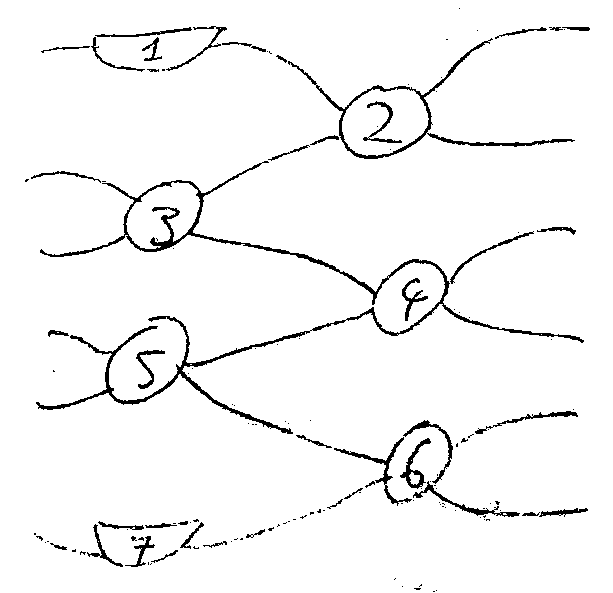
\includegraphics[scale=0.2]{network}
	\hspace{3em}
	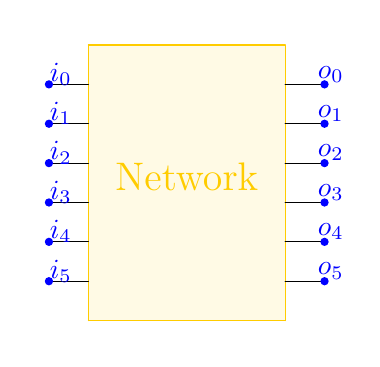
\begin{tikzpicture}[line cap=round,line join=round,>=triangle 45,x=0.5cm,y=0.5cm]
		\clip(0.46,-5.46) rectangle (8.7,2.44);
			\fill[color=ffccqq,fill=ffccqq,fill opacity=0.1] (2,2) -- (7,2) -- (7,-5) -- (2,-5) -- cycle;
			\draw [color=ffccqq] (2,2)-- (7,2);
			\draw [color=ffccqq] (7,2)-- (7,-5);
			\draw [color=ffccqq] (7,-5)-- (2,-5);
			\draw [color=ffccqq] (2,-5)-- (2,2);
		\draw (1,1)-- (2,1);
		\draw (1,0)-- (2,0);
		\draw (1,-1)-- (2,-1);
		\draw (1,-2)-- (2,-2);
		\draw (1,-3)-- (2,-3);
		\draw (1,-4)-- (2,-4);
		\draw (7,-4)-- (8,-4);
		\draw (7,-3)-- (8,-3);
		\draw (7,-2)-- (8,-2);
		\draw (7,-1)-- (8,-1);
		\draw (7,0)-- (8,0);
		\draw (7,1)-- (8,1);
		\fill [color=qqqqff] (1,1) circle (1.5pt);
			\draw[color=qqqqff] (1.3,1.26) node {$i_0$};
		\fill [color=qqqqff] (1,0) circle (1.5pt);
			\draw[color=qqqqff] (1.3,0.26) node {$i_1$};
		\fill [color=qqqqff] (1,-1) circle (1.5pt);
			\draw[color=qqqqff] (1.3,-0.74) node {$i_2$};
		\fill [color=qqqqff] (1,-2) circle (1.5pt);
			\draw[color=qqqqff] (1.3,-1.74) node {$i_3$};
		\fill [color=qqqqff] (1,-3) circle (1.5pt);
			\draw[color=qqqqff] (1.3,-2.74) node {$i_4$};
		\fill [color=qqqqff] (1,-4) circle (1.5pt);
			\draw[color=qqqqff] (1.3,-3.74) node {$i_5$};
		\fill [color=qqqqff] (8,-4) circle (1.5pt);
			\draw[color=qqqqff] (8.16,-3.74) node {$o_5$};
		\fill [color=qqqqff] (8,-3) circle (1.5pt);
			\draw[color=qqqqff] (8.16,-2.74) node {$o_4$};
		\fill [color=qqqqff] (8,-2) circle (1.5pt);
			\draw[color=qqqqff] (8.16,-1.74) node {$o_3$};
		\fill [color=qqqqff] (8,-1) circle (1.5pt);
			\draw[color=qqqqff] (8.16,-0.74) node {$o_2$};
		\fill [color=qqqqff] (8,0) circle (1.5pt);
			\draw[color=qqqqff] (8.16,0.26) node {$o_1$};
		\fill [color=qqqqff] (8,1) circle (1.5pt);
			\draw[color=qqqqff] (8.16,1.26) node {$o_0$};
		\draw[color=ffccqq] (4.5,-1.34) node {\Large Network};
	\end{tikzpicture}
	\end{center}

\end{frame}


\section{Examples in the case $k=3$}
% ===================================================================

\begin{frame}{3 functions in base 3}
	We managed to compute 3 "interesting" functions in base 3 over DNA-nanotube network:\pause
		
	\begin{itemize}
		\item a indicator of 1\pause
		\item a counter of 1's mod 3\pause
		\item a binary additioner (using base 3 network!)
	\end{itemize}
\end{frame}

\subsection{The 1 indicator}
% --------------------------------------------------------------------

\begin{frame}{The "1 indicator"}
	
	This function outputs $o_0$ = 1 iff there some $i_j$ = 1 (others outputs are always 0).
	\pause
	To do it, we used these cells:
	
	\begin{center}
	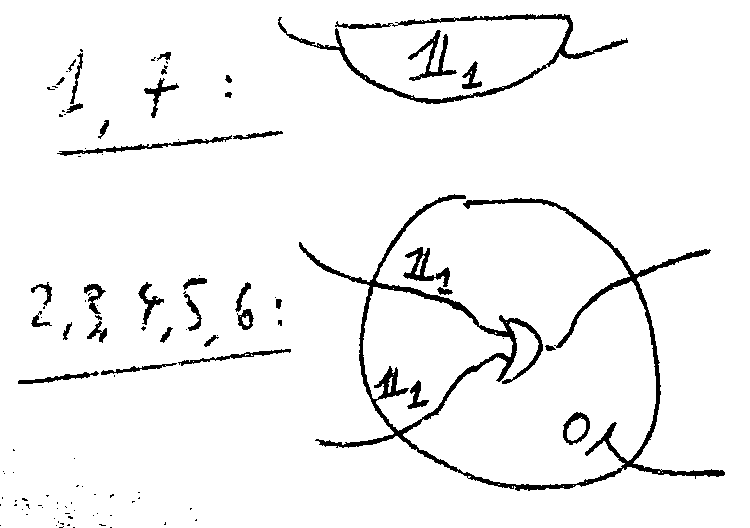
\includegraphics[scale=0.2]{1indicator_settings}
	\hspace{2em}
	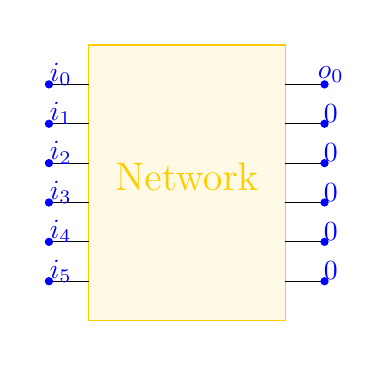
\begin{tikzpicture}[line cap=round,line join=round,>=triangle 45,x=0.5cm,y=0.5cm]
		\clip(0.46,-5.46) rectangle (9,2.44);
			\fill[color=ffccqq,fill=ffccqq,fill opacity=0.1] (2,2) -- (7,2) -- (7,-5) -- (2,-5) -- cycle;
			\draw [color=ffccqq] (2,2)-- (7,2);
			\draw [color=ffccqq] (7,2)-- (7,-5);
			\draw [color=ffccqq] (7,-5)-- (2,-5);
			\draw [color=ffccqq] (2,-5)-- (2,2);
		\draw (1,1)-- (2,1);
		\draw (1,0)-- (2,0);
		\draw (1,-1)-- (2,-1);
		\draw (1,-2)-- (2,-2);
		\draw (1,-3)-- (2,-3);
		\draw (1,-4)-- (2,-4);
		\draw (7,-4)-- (8,-4);
		\draw (7,-3)-- (8,-3);
		\draw (7,-2)-- (8,-2);
		\draw (7,-1)-- (8,-1);
		\draw (7,0)-- (8,0);
		\draw (7,1)-- (8,1);
		\fill [color=qqqqff] (1,1) circle (1.5pt);
			\draw[color=qqqqff] (1.3,1.26) node {$i_0$};
		\fill [color=qqqqff] (1,0) circle (1.5pt);
			\draw[color=qqqqff] (1.3,0.26) node {$i_1$};
		\fill [color=qqqqff] (1,-1) circle (1.5pt);
			\draw[color=qqqqff] (1.3,-0.74) node {$i_2$};
		\fill [color=qqqqff] (1,-2) circle (1.5pt);
			\draw[color=qqqqff] (1.3,-1.74) node {$i_3$};
		\fill [color=qqqqff] (1,-3) circle (1.5pt);
			\draw[color=qqqqff] (1.3,-2.74) node {$i_4$};
		\fill [color=qqqqff] (1,-4) circle (1.5pt);
			\draw[color=qqqqff] (1.3,-3.74) node {$i_5$};
		\fill [color=qqqqff] (8,-4) circle (1.5pt);
			\draw[color=qqqqff] (8.16,-3.74) node {0};
		\fill [color=qqqqff] (8,-3) circle (1.5pt);
			\draw[color=qqqqff] (8.16,-2.74) node {0};
		\fill [color=qqqqff] (8,-2) circle (1.5pt);
			\draw[color=qqqqff] (8.16,-1.74) node {0};
		\fill [color=qqqqff] (8,-1) circle (1.5pt);
			\draw[color=qqqqff] (8.16,-0.74) node {0};
		\fill [color=qqqqff] (8,0) circle (1.5pt);
			\draw[color=qqqqff] (8.16,0.26) node {0};
		\fill [color=qqqqff] (8,1) circle (1.5pt);
			\draw[color=qqqqff] (8.16,1.26) node {$o_0$};
		\draw[color=ffccqq] (4.5,-1.34) node {\Large Network};
	\end{tikzpicture}
	\end{center}
\end{frame}

\subsection{Counting 1's mod 3}
% --------------------------------------------------------------------

\begin{frame}{The counter of 1's mod 3}
	
	This functions computes the number of ones in the input and sets $o_0$,$o_1$ (which must be a fixed point for the function). Other outputs are always 0.
	
	\pause
	
	\begin{center}
	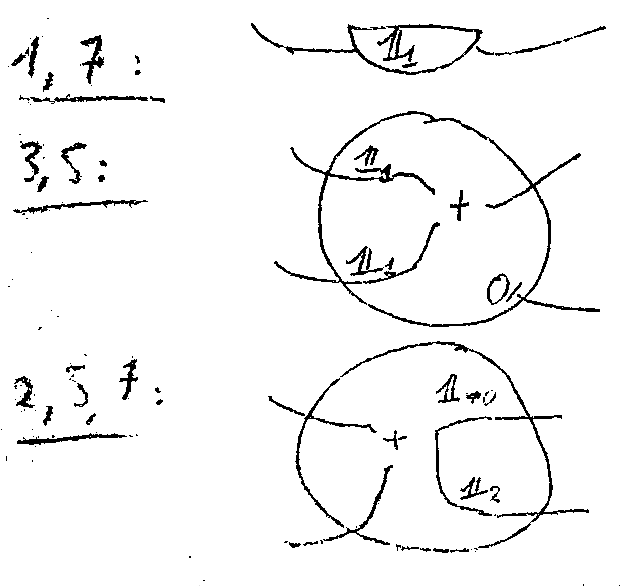
\includegraphics[scale=0.2]{1counter_mod3}
	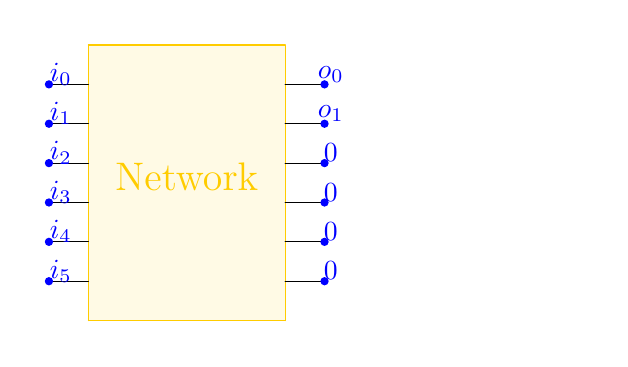
\begin{tikzpicture}[line cap=round,line join=round,>=triangle 45,x=0.5cm,y=0.5cm]
		\clip(0.46,-5.46) rectangle (15,2.44);
			\fill[color=ffccqq,fill=ffccqq,fill opacity=0.1] (2,2) -- (7,2) -- (7,-5) -- (2,-5) -- cycle;
			\draw [color=ffccqq] (2,2)-- (7,2);
			\draw [color=ffccqq] (7,2)-- (7,-5);
			\draw [color=ffccqq] (7,-5)-- (2,-5);
			\draw [color=ffccqq] (2,-5)-- (2,2);
		\draw (1,1)-- (2,1);
		\draw (1,0)-- (2,0);
		\draw (1,-1)-- (2,-1);
		\draw (1,-2)-- (2,-2);
		\draw (1,-3)-- (2,-3);
		\draw (1,-4)-- (2,-4);
		\draw (7,-4)-- (8,-4);
		\draw (7,-3)-- (8,-3);
		\draw (7,-2)-- (8,-2);
		\draw (7,-1)-- (8,-1);
		\draw (7,0)-- (8,0);
		\draw (7,1)-- (8,1);
		\fill [color=qqqqff] (1,1) circle (1.5pt);
			\draw[color=qqqqff] (1.3,1.26) node {$i_0$};
		\fill [color=qqqqff] (1,0) circle (1.5pt);
			\draw[color=qqqqff] (1.3,0.26) node {$i_1$};
		\fill [color=qqqqff] (1,-1) circle (1.5pt);
			\draw[color=qqqqff] (1.3,-0.74) node {$i_2$};
		\fill [color=qqqqff] (1,-2) circle (1.5pt);
			\draw[color=qqqqff] (1.3,-1.74) node {$i_3$};
		\fill [color=qqqqff] (1,-3) circle (1.5pt);
			\draw[color=qqqqff] (1.3,-2.74) node {$i_4$};
		\fill [color=qqqqff] (1,-4) circle (1.5pt);
			\draw[color=qqqqff] (1.3,-3.74) node {$i_5$};
		\fill [color=qqqqff] (8,-4) circle (1.5pt);
			\draw[color=qqqqff] (8.16,-3.74) node {0};
		\fill [color=qqqqff] (8,-3) circle (1.5pt);
			\draw[color=qqqqff] (8.16,-2.74) node {0};
		\fill [color=qqqqff] (8,-2) circle (1.5pt);
			\draw[color=qqqqff] (8.16,-1.74) node {0};
		\fill [color=qqqqff] (8,-1) circle (1.5pt);
			\draw[color=qqqqff] (8.16,-0.74) node {0};
		\fill [color=qqqqff] (8,0) circle (1.5pt);
			\draw[color=qqqqff] (8.16,0.26) node {$o_1$};
		\fill [color=qqqqff] (8,1) circle (1.5pt);
			\draw[color=qqqqff] (8.16,1.26) node {$o_0$};
		\draw[color=ffccqq] (4.5,-1.34) node {\Large Network};
	\end{tikzpicture}
	\end{center}
\end{frame}

\subsection{A binary additioner}
% --------------------------------------------------------------------

\begin{frame}{Binary additioner: What it does...}
	Given 2 binary inputs of length 3 ($i_{0}i_{2}i_{4}$ and $i_{1}i_{3}i_{5}$), this function computes the sum mod 8 on outputs $o_{1}o_{3}o_{5}$ (other outputs are set to 0).
	
	\begin{center}
	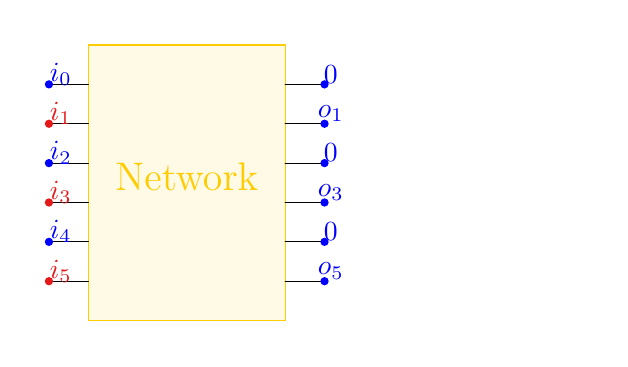
\begin{tikzpicture}[line cap=round,line join=round,>=triangle 45,x=0.5cm,y=0.5cm]
		\clip(0.46,-5.46) rectangle (15,2.44);
			\fill[color=ffccqq,fill=ffccqq,fill opacity=0.1] (2,2) -- (7,2) -- (7,-5) -- (2,-5) -- cycle;
			\draw [color=ffccqq] (2,2)-- (7,2);
			\draw [color=ffccqq] (7,2)-- (7,-5);
			\draw [color=ffccqq] (7,-5)-- (2,-5);
			\draw [color=ffccqq] (2,-5)-- (2,2);
		\draw (1,1)-- (2,1);
		\draw (1,0)-- (2,0);
		\draw (1,-1)-- (2,-1);
		\draw (1,-2)-- (2,-2);
		\draw (1,-3)-- (2,-3);
		\draw (1,-4)-- (2,-4);
		\draw (7,-4)-- (8,-4);
		\draw (7,-3)-- (8,-3);
		\draw (7,-2)-- (8,-2);
		\draw (7,-1)-- (8,-1);
		\draw (7,0)-- (8,0);
		\draw (7,1)-- (8,1);
		\fill [color=qqqqff] (1,1) circle (1.5pt);
			\draw[color=qqqqff] (1.3,1.26) node {$i_0$};
		\fill [color=ffqqqq] (1,0) circle (1.5pt);
			\draw[color=ffqqqq] (1.3,0.26) node {$i_1$};
		\fill [color=qqqqff] (1,-1) circle (1.5pt);
			\draw[color=qqqqff] (1.3,-0.74) node {$i_2$};
		\fill [color=ffqqqq] (1,-2) circle (1.5pt);
			\draw[color=ffqqqq] (1.3,-1.74) node {$i_3$};
		\fill [color=qqqqff] (1,-3) circle (1.5pt);
			\draw[color=qqqqff] (1.3,-2.74) node {$i_4$};
		\fill [color=ffqqqq] (1,-4) circle (1.5pt);
			\draw[color=ffqqqq] (1.3,-3.74) node {$i_5$};
		\fill [color=qqqqff] (8,-4) circle (1.5pt);
			\draw[color=qqqqff] (8.16,-3.74) node {$o_5$};
		\fill [color=qqqqff] (8,-3) circle (1.5pt);
			\draw[color=qqqqff] (8.16,-2.74) node {0};
		\fill [color=qqqqff] (8,-2) circle (1.5pt);
			\draw[color=qqqqff] (8.16,-1.74) node {$o_3$};
		\fill [color=qqqqff] (8,-1) circle (1.5pt);
			\draw[color=qqqqff] (8.16,-0.74) node {0};
		\fill [color=qqqqff] (8,0) circle (1.5pt);
			\draw[color=qqqqff] (8.16,0.26) node {$o_1$};
		\fill [color=qqqqff] (8,1) circle (1.5pt);
			\draw[color=qqqqff] (8.16,1.26) node {0};
		\draw[color=ffccqq] (4.5,-1.34) node {\Large Network};
	\end{tikzpicture}
	\end{center}
\end{frame}

\begin{frame}{... and how it works}
	\begin{center}
	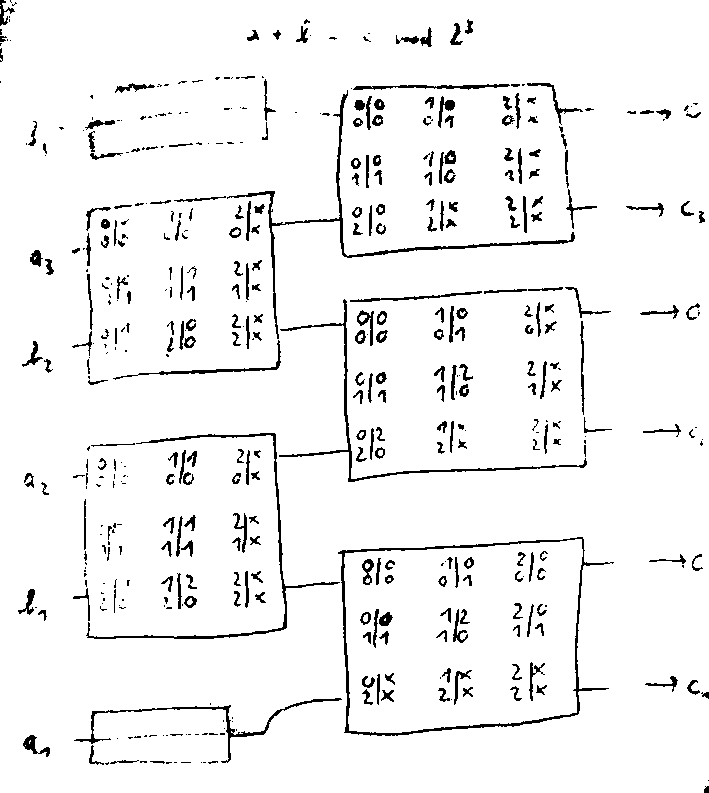
\includegraphics[scale=0.23]{binary_additioner}
	\end{center}
\end{frame}


\section{Compiling the network into tiles}
% ===================================================================

\begin{frame}{Compiling the network into tiles}
	\begin{center}
		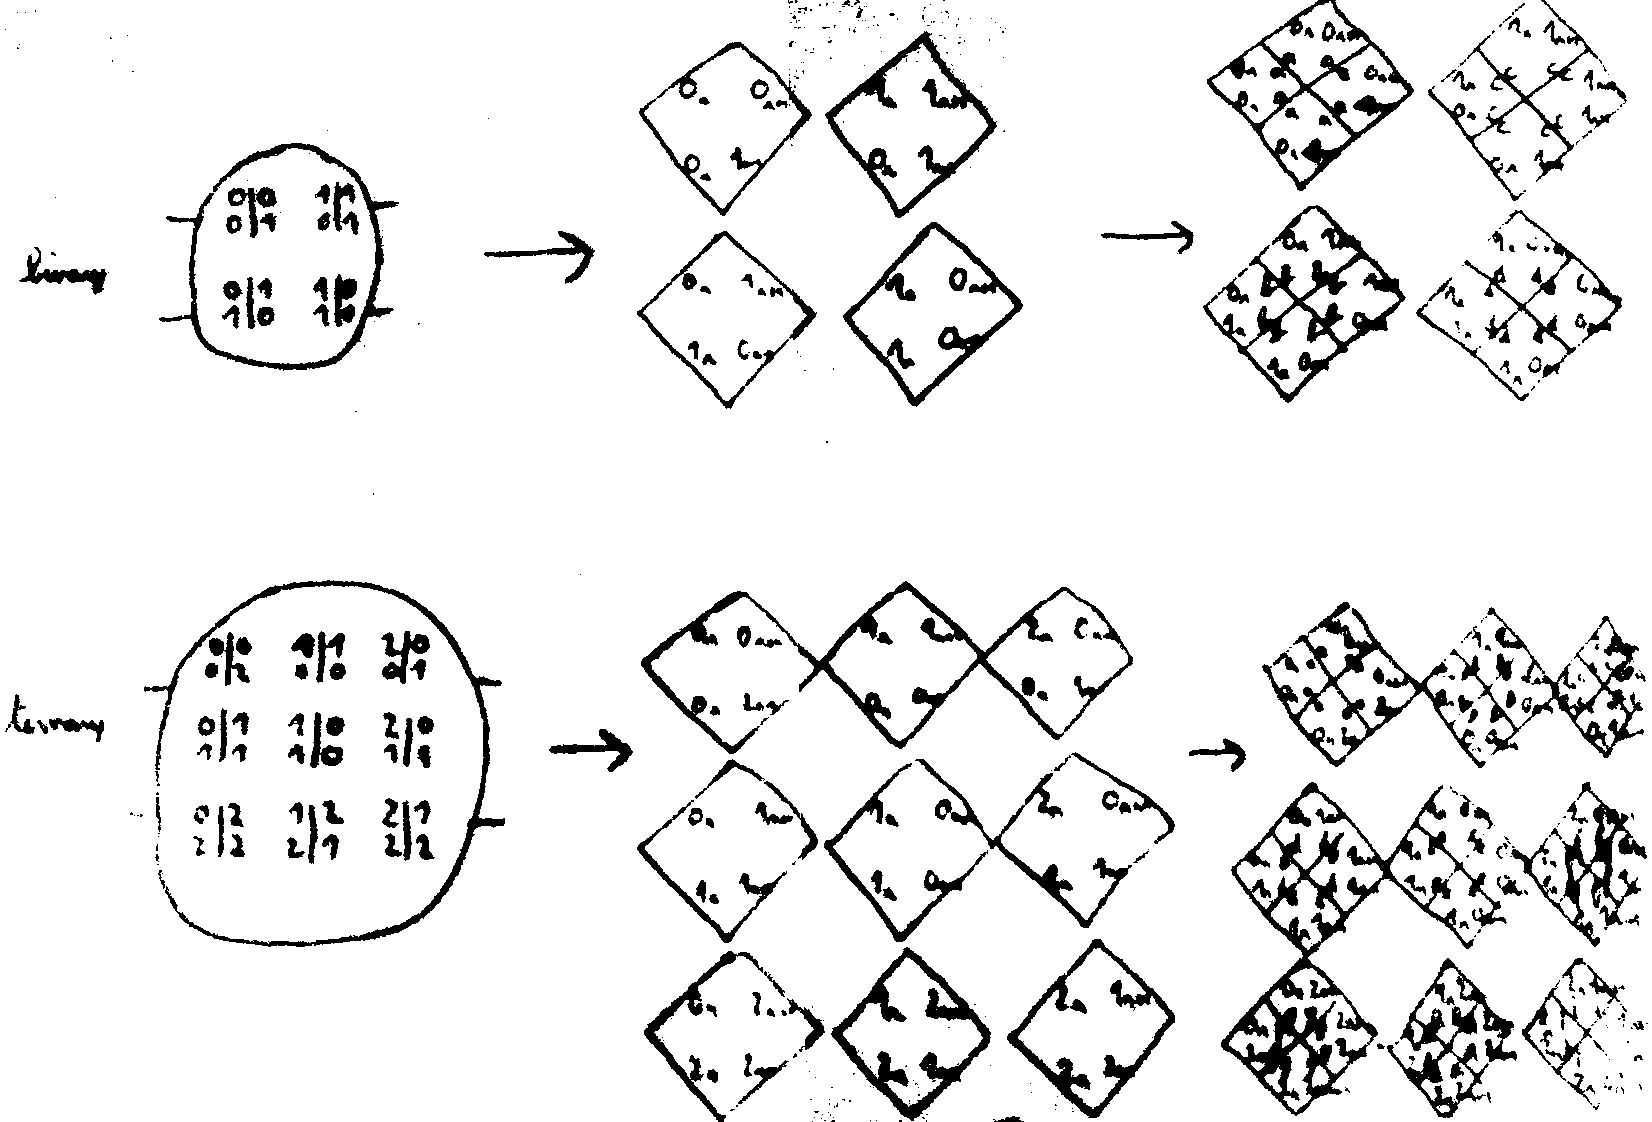
\includegraphics[scale=0.15]{compile}
	\end{center}
\end{frame}

\begin{frame}{Represent circuit as a graph.}
	We have 7 possible positions and we have $k^2$ possible tile choice for each.
	
	\begin{center}
		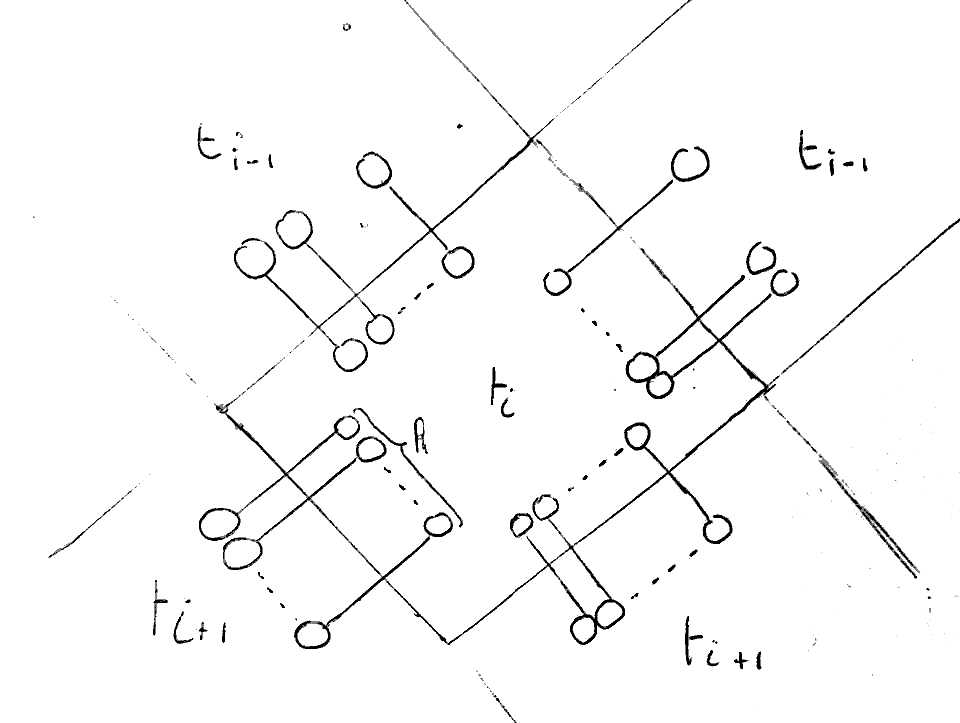
\includegraphics[scale=0.18]{tograph}
	\end{center}
	Each time a tile can be placed next to an other their colors become linked.
\end{frame}

\begin{frame}{Convert tiles into proofreading tiles}
	We add 8 new colors per tile and all the previous colors were replaced by two new colors.
	\begin{center}
		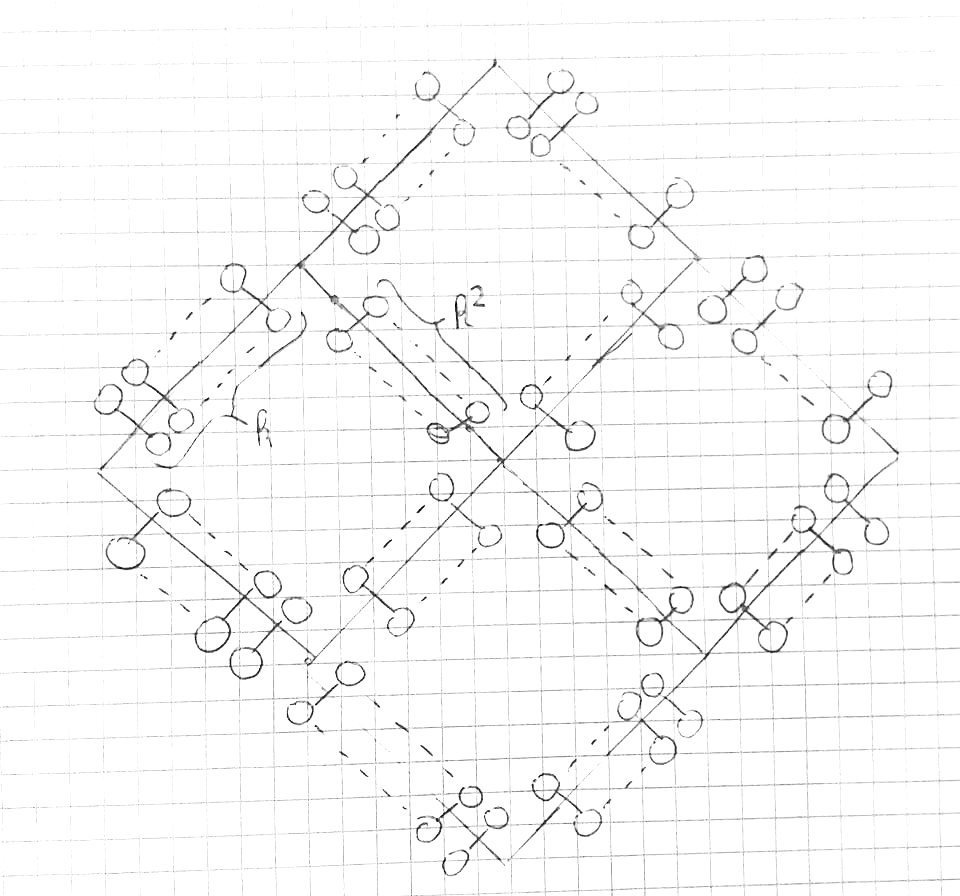
\includegraphics[scale=0.12]{proofreading}
	\end{center}
	\pause
	Each color will be associated to a DNA-string of size fixed $L$.
	Each tile will be the concatenation of it's 4 colors.
\end{frame}

\section{Looking for a 6 bit counter}
% ===================================================================


\subsection{Problem Statement}
% --------------------------------------------------------------------

\begin{frame}{Does a 6 bit counter exists?} 
	Can we create a \textbf{deterministic} network that will iterate over all 6 bits string --- in any order?
\end{frame}

\begin{frame}{Does a 6 bit counter exists ?} 
	\centering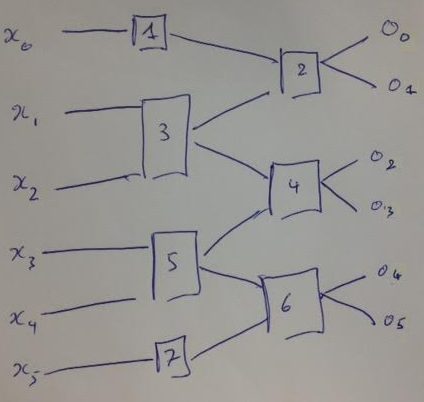
\includegraphics[scale=0.55]{netk.png}
\end{frame}


\begin{frame}{Can we bruteforce that problem ?}
	There are $\boldsymbol{2^{44}}$ differents networks which is approximatively $17 000$ billions.
	
	We could hope for an answer in a few days.
	
	\textbf{But} we can drastically restrict our search space with a \textbf{few} observations.
	\bigskip\pause
	
	\textbf{Main ideas :} 
	\begin{itemize}
	\item Get rid of \textbf{redundancy}
	\item Look at interesting \textbf{sub-networks}
	\end{itemize}
\end{frame} 

\begin{frame}{6bit Networks are HUGELY redundant}
	There are $\boldsymbol{2^{44}}$ differents networks which is approximatively $17 000$ billions. \\ \ \\
	
	But these networks allow to compute only about \textbf{32 billions} different layer functions. \\ \ \\
	So there is only about \textbf{0.2\%} interesting networks in the sense that they compute distinct layer functions. \\ \ \\
	This model allows to calculate on a layer only \textbf{8.2e-104 \%} of all functions of $\{0,1\}^6 \rightarrow \{0,1\}^6$ (there are $64^{64}$).
\end{frame} 


\begin{frame}{How would such a network's dynamic look like ?} 
	There are only two possibilities (up to permutation):
	
	\centering\rotatebox{180}{
		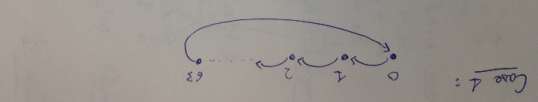
\includegraphics[scale=0.45]{2cases.png}
	}\medskip\pause
	
	\centering\rotatebox{180}{
		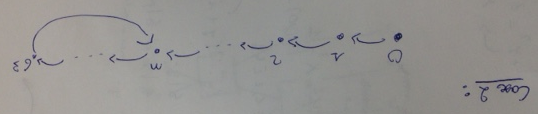
\includegraphics[scale=0.45]{2cases2.png}
	}
\end{frame}

\begin{frame}{Implication on the layer function of the network} 
	The function that our counting network coumputes on one layer is either:
	\begin{itemize}
		\item \textbf{A bijection}
		\item \textbf{An almost-bijection}\pause{} i.e. $f$ such that $\exists ! x_0,y_0 \in \{0,1\}^6$ with $f'$ being a bijection and:  
		\begin{align*}
			\forall x \neq x_0 \quad & f'(x) = f(x)  \\
								     & f'(x_0) = y_0 \\
		\end{align*}
	\end{itemize}\pause
	We are going to check on both cases.
\end{frame}

\subsection{Computable bijections on $\{0,1\}^6$ and 4*16 rule}
% --------------------------------------------------------------------

\begin{frame}{The $4*16$ property} 
	If we have a bijection it will \textbf{enumerate} all strings of  
	$\{0,1\}^6$. After reordering it will look like:
	\medskip
	
	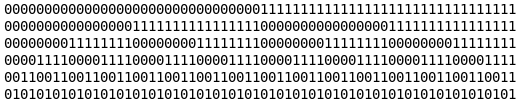
\includegraphics[scale=0.6]{all6b.png}
\end{frame}

\begin{frame}{The $4*16$ property} 
	Let's focus on the first two bits, we can organise our sequences this way:
	\medskip
	
	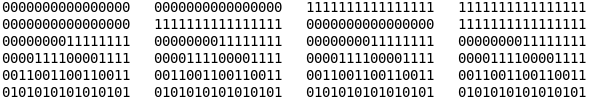
\includegraphics[scale=0.55]{all6b2b.png}
\end{frame}

\begin{frame}{The $4*16$ property} 
	Let us get rid of the last 4 bits:
	\medskip
	
	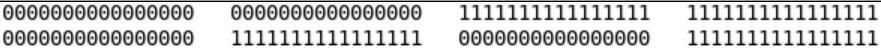
\includegraphics[scale=0.45]{6b2b.png}
	\medskip\pause
	
	We see that each of the 2 bits patterns:  \textbf{00, 01, 10, 11} occurs \textbf{16} times in this enumeration.\\
	It's the \textbf{$\boldsymbol{4*16}$ property}.
\end{frame}

\begin{frame}{The $4*16$ property} 
	\textbf{Hence} the sub network responsible for these 2 bits must have the \textbf{4*16} property to be eligible as a being a sub network of a 6 bits bijective counter network.
	\medskip\pause
	
	\centering\rotatebox{90}{
		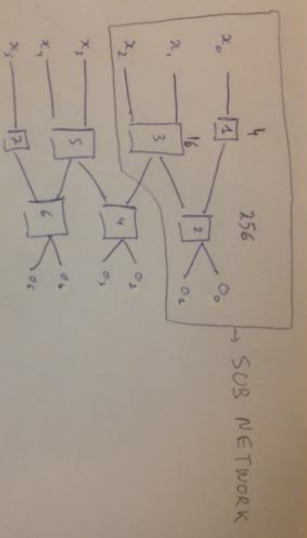
\includegraphics[scale=0.56]{subnetk.png}
	}
\end{frame}

\begin{frame}{Compute all the $4*16$ sub networks} 
	By exausthive search we find $\boldsymbol{288}$ (over $4*16*256=16384$) sub networks with this property.\medskip
	
	By removing equivalent networks we are left with \textbf{$\boldsymbol{72}$ circuits for the first 2 bits}.
\end{frame}

\begin{frame}{4*16 holds for middle and ending bits}	
	\centering\rotatebox{90}{
		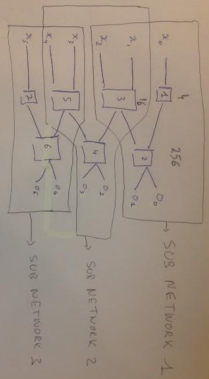
\includegraphics{subnetsk.png}
	}
\end{frame}

\begin{frame}{4*16 holds for middle and ending bits}
	\begin{itemize}
		\item \textbf{72} networks for the first 2 bits
		\item \textbf{216} networks for the middle 2 bits
		\item \textbf{72} networks for the last 2 bits
	\end{itemize}
\end{frame}

\begin{frame}{How to conclude? --- 1. Combine it!}
	\textbf{Hence} by combining these we have $72*216*72 \simeq 10^6$ \\ 6 bits networks to test.
\end{frame} 

\begin{frame}{How to conclude? --- 2. Count orbits!}
	Over all these potential networks we count $\boldsymbol{497664}$ bijections. \\
	For each of these bijections we have to \textbf{count their orbits}, we have a winner \textbf{iff it has only 1 orbit}.
	\medskip\pause
	
	We do not find such a network, here there's the histogram of orbits:
	
	\centering
	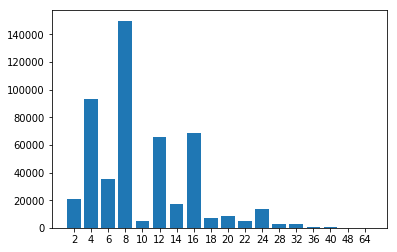
\includegraphics[scale=0.46]{hist_orbits.png}
\end{frame} 

\begin{frame}{Conclusion}
	\textbf{Conclusion:} There are no bijective 6bits counters.
\end{frame}


\subsection{Computable almost-bijections on $\{0,1\}^6$}
% --------------------------------------------------------------------

\begin{frame}{2*161517 property}
	If we have an almost-bijection \textbf{all 6 bits sequences will be reached by our network but one}.\medskip\pause
	
	Also one bit string will be reached \textbf{twice}. \medskip\pause
	
	It means that \textbf{at least one} of our sub network will see:
	\begin{itemize}
		\item 2 patterns \textbf{16} times
		\item 1 pattern \textbf{15} times
		\item 1 pattern \textbf{17} times
	\end{itemize}\pause\bigskip

	We call this the \textbf{2*161517 property}.
\end{frame}

\begin{frame}{2*161517 does not occur!}
	By enumeration, \textbf{there exist no sub network with the 2*161517} property. \\
	\textbf{Hence}, we cannot hope for an \textbf{almost-bijective counter}.
\end{frame}

\subsection{Conclusion and perspectives}
% --------------------------------------------------------------------

\begin{frame}{No 6bit counter network :'( }
	By case distinction, \textbf{there's no 6bit counter network}.
	\medskip\pause
	
	But there are \textbf{0 to 62} counters and this kind of methods helps to exhibit \textbf{at least 24}.
\end{frame}

\begin{frame}{Perspectives}
	\begin{itemize}

		\item The fact that no sub-network has the 2x161517 property helps to find an argument for a \textbf{formal proof} in the almost-bijective case.
		\item We saw that our network model was hugely redundant. To make formal proof it would nice if we could find a \textbf{canonical} form for each network. 
	\end{itemize}
\end{frame}

\begin{frame}{Sources}
	All our sources for these computations are available here:
	\url{https://github.com/cosmo-sterin/ER_MolProg_Project2/tree/master/circuit_sim}
\end{frame}

\end{document}
